%%%% Proceedings format for most of ACM conferences (with the exceptions listed below) and all ICPS volumes.
\documentclass[sigconf]{acmart}
%%%% As of March 2017, [siggraph] is no longer used. Please use sigconf (above) for SIGGRAPH conferences.

%%%% Proceedings format for SIGPLAN conferences 
% \documentclass[sigplan, anonymous, review]{acmart}

%%%% Proceedings format for SIGCHI conferences
% \documentclass[sigchi, review]{acmart}

%%%% To use the SIGCHI extended abstract template, please visit
% https://www.overleaf.com/read/zzzfqvkmrfzn
\usepackage{float}
\usepackage{multirow}
\usepackage[normalem]{ulem}
\useunder{\uline}{\ul}{}
%
% defining the \BibTeX command - from Oren Patashnik's original BibTeX documentation.
\def\BibTeX{{\rm B\kern-.05em{\sc i\kern-.025em b}\kern-.08emT\kern-.1667em\lower.7ex\hbox{E}\kern-.125emX}}
    
% Rights management information. 
% This information is sent to you when you complete the rights form.
% These commands have SAMPLE values in them; it is your responsibility as an author to replace
% the commands and values with those provided to you when you complete the rights form.
%
% These commands are for a PROCEEDINGS abstract or paper.


\copyrightyear{2020} 
\acmYear{2020} 
\acmConference[MM '20]{Proceedings of the 28th ACM International Conference on Multimedia}{October 12--16, 2020}{Seattle, United States}
\acmBooktitle{Proceedings of the 28th ACM International Conference on Multimedia (MM '20), October 12--16, 2020, Seattle, United States}
\acmPrice{15.00}
\acmDOI{10.1145/3343031.3351016}
\acmISBN{978-1-4503-6889-6/19/10}
\setcopyright{acmcopyright}
%
% These commands are for a JOURNAL article.
%\setcopyright{acmcopyright}
%\acmJournal{TOG}
%\acmYear{2018}\acmVolume{37}\acmNumber{4}\acmArticle{111}\acmMonth{8}
%\acmDOI{10.1145/1122445.1122456}

%
% Submission ID. 
% Use this when submitting an article to a sponsored event. You'll receive a unique submission ID from the organizers
% of the event, and this ID should be used as the parameter to this command.
%\acmSubmissionID{123-A56-BU3}

%
% The majority of ACM publications use numbered citations and references. If you are preparing content for an event
% sponsored by ACM SIGGRAPH, you must use the "author year" style of citations and references. Uncommenting
% the next command will enable that style.
%\citestyle{acmauthoryear}

%
% end of the preamble, start of the body of the document source.
\begin{document}

%
% The "title" command has an optional parameter, allowing the author to define a "short title" to be used in page headers.
\title{Disentangled High-Resolution Salient Object Detection}
\subtitle{Submission 1526}
%
% The "author" command and its associated commands are used to define the authors and their affiliations.
% Of note is the shared affiliation of the first two authors, and the "authornote" and "authornotemark" commands
% used to denote shared contribution to the research.
%\author{Ben Trovato}
%\authornote{Both authors contributed equally to this research.}
%\email{trovato@corporation.com}
%\orcid{1234-5678-9012}
%\author{G.K.M. Tobin}
%\authornotemark[1]
%\email{webmaster@marysville-ohio.com}
%\affiliation{%
%  \institution{Institute for Clarity in Documentation}
%  \streetaddress{P.O. Box 1212}
%  \city{Dublin}
%  \state{Ohio}
%  \postcode{43017-6221}
%}

%\author{Lars Th{\o}rv{\"a}ld}
%\affiliation{%
 % \institution{The Th{\o}rv{\"a}ld Group}
  %\streetaddress{1 Th{\o}rv{\"a}ld Circle}
  %\city{Hekla}
  %\country{Iceland}}
%\email{larst@affiliation.org}

%\author{Valerie B\'eranger}
%\affiliation{%
 % \institution{Inria Paris-Rocquencourt}
  %\city{Rocquencourt}
  %\country{France}
%}

 
%\author{Huifen Chan}
%\affiliation{%
%  \institution{Tsinghua University}
%  \streetaddress{30 Shuangqing Rd}
%  \city{Haidian Qu}
%  \state{Beijing Shi}
%  \country{China}}


%\author{John Smith}
%\affiliation{\institution{The Th{\o}rv{\"a}ld Group}}
%\email{jsmith@affiliation.org}

%\author{Julius P. Kumquat}
%\affiliation{\institution{The Kumquat Consortium}}
%\email{jpkumquat@consortium.net}

%
% By default, the full list of authors will be used in the page headers. Often, this list is too long, and will overlap
% other information printed in the page headers. This command allows the author to define a more concise list
% of authors' names for this purpose.
\renewcommand{\shortauthors}{Trovato and Tobin, et al.}

%
% The abstract is a short summary of the work to be presented in the article.
\begin{abstract}
As an interesting and emerging topic, co-saliency detection aims at discovering common and salient objects in a group of related images, which is  useful  to  variety  of  visual media applications. Although a number of approaches have been proposed to address this problem, many of them are designed with the misleading assumption, suboptimal image representation, or heavy supervision cost and thus still suffer from certain limitations, which reduces their capability in the real-world scenarios. To alleviate these limitations, we propose a novel unsupervised co-saliency detection method, which successively explores the hierarchical consistency in the image group including background consistency, high-level and low-level objects consistency in a unified framework. We first design a novel superpixel-wise variational autoencoder (SVAE) network to precisely distinguish the salient objects from the background collection based on the reconstruction errors. Then, we propose a two-stage clustering strategy to explore the multi-level salient objects consistency by using high-level and low-level features separately. Finally, the co-saliency results are refined by applying a CRF based refinement method with the multi-level salient objects consistency. Extensive experiments on three widely datasets show that our method achieves superior or competitive performance compared to the state-of-the-art methods.
\end{abstract}

%
% The code below is generated by the tool at http://dl.acm.org/ccs.cfm.
% Please copy and paste the code instead of the example below.
%
\begin{CCSXML}
<ccs2012>
<concept>
<concept_id>10010147.10010178.10010224.10010245.10010247</concept_id>
<concept_desc>Computing methodologies~Image segmentation</concept_desc>
<concept_significance>500</concept_significance>
</concept>
</ccs2012>
\end{CCSXML}

\ccsdesc[500]{Computing methodologies~Image segmentation}

%
% Keywords. The author(s) should pick words that accurately describe the work being
% presented. Separate the keywords with commas.
\keywords{Co-saliency detection, variational autoencoder (VAE), Deep learning, Clustering }

%
% A "teaser" image appears between the author and affiliation information and the body 
% of the document, and typically spans the page. 
%\begin{teaserfigure}
%  \includegraphics[width=\textwidth]{sampleteaser}
%  \caption{Seattle Mariners at Spring Training, 2010.}
%  \Description{Enjoying the baseball game from the third-base seats. Ichiro Suzuki preparing to bat.}
%  \label{fig:teaser}
%\end{teaserfigure}

%
% This command processes the author and affiliation and title information and builds
% the first part of the formatted document.
\maketitle

\section{Introduction}

Salient object detection is derived with the goal of accurately detecting and segmenting the most distinctive objects from visual scenes. As a preliminary step, it plays an essential role in various visual media  systems, such as semantic segmentation \cite{DBLP:journals/pami/WeiLCSCFZY17}, 
image quality assessment\cite{DBLP:conf/mm/YangJLW19},
360-degree head-mounted display\cite{DBLP:conf/mm/NguyenYN18},
light field 3D display\cite{DBLP:conf/cvpr/WangLS0ZY18}
 and image-sentence matching \cite{Ji_2019_ICCV}.
 
 \begin{figure}[!t]
\centering
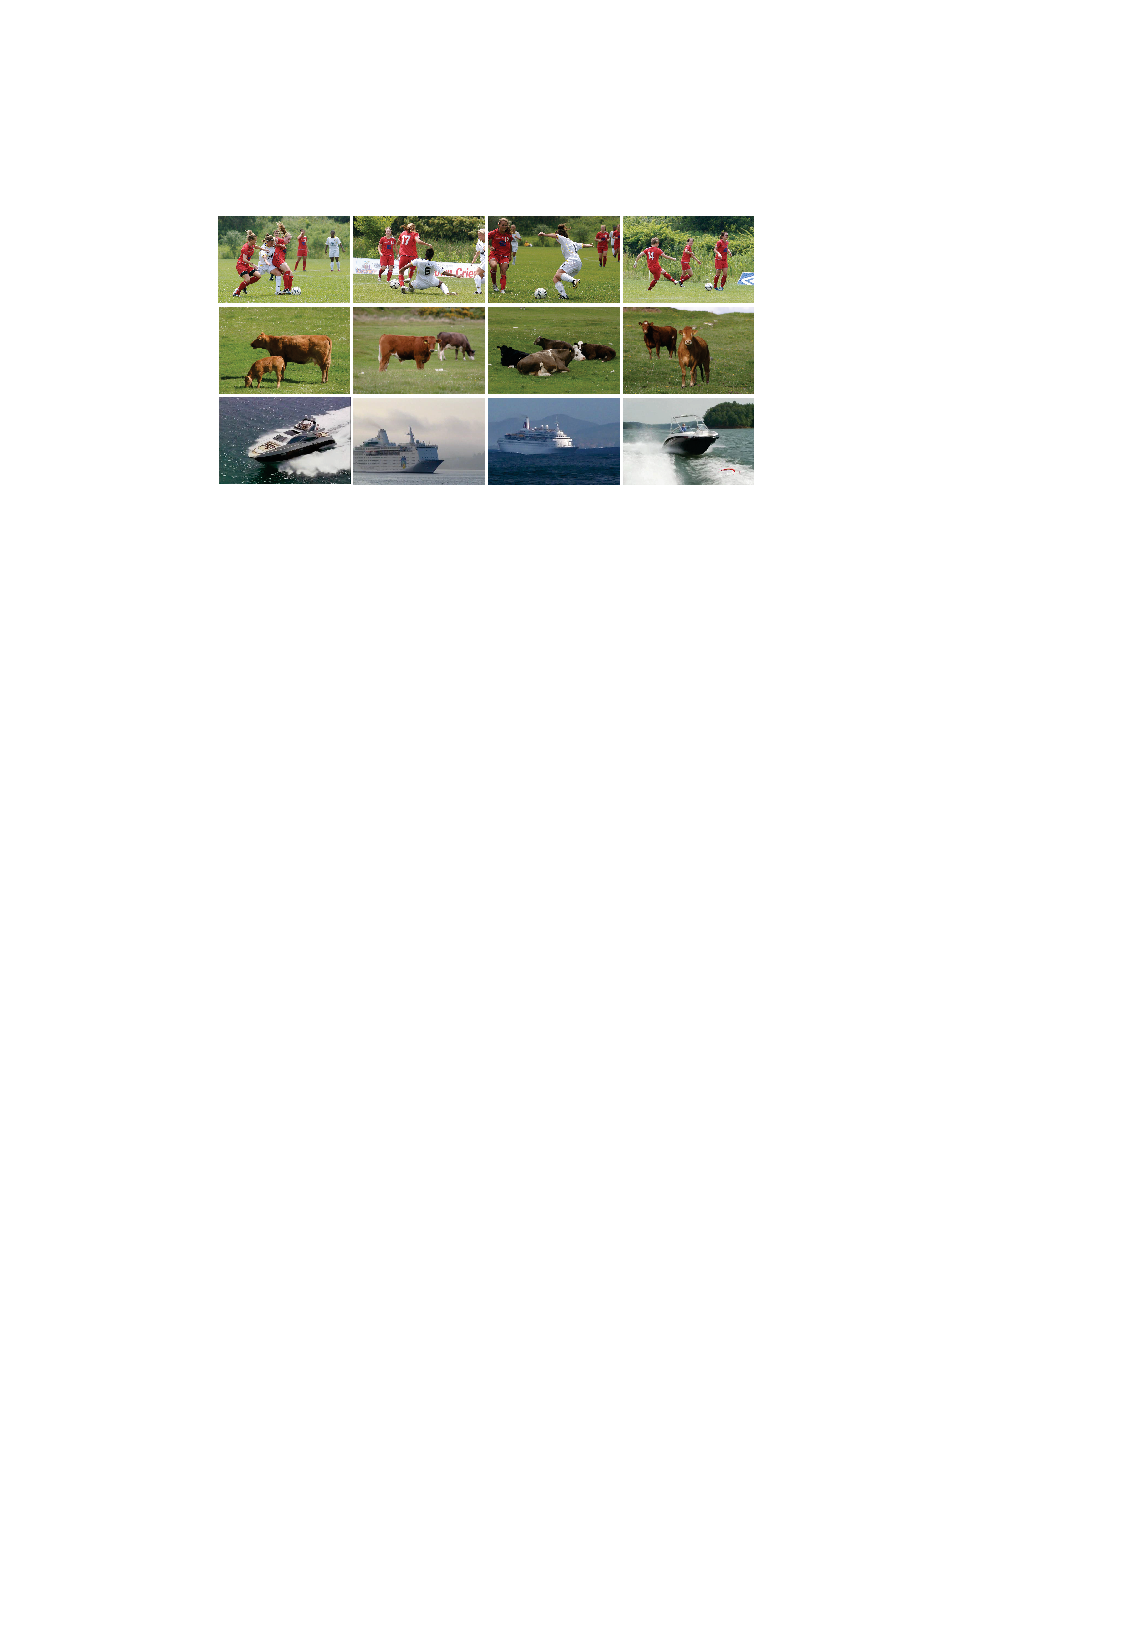
\includegraphics[scale=0.9,width = 8.5cm]{Fig1.pdf}
\caption{Examples illustrating the common objects within an image group usually occur in related scenes.The images in the same row belong to the same group.}
\label{fig:label}
\end{figure}

 
Recently, the rapid development of the commodity imaging and display device, have resulted in higher requirements for the producing and editing of high-resolution (e.g., 720p, 1080p and 4K) visual media. Salient object detection as well as many state-of-the-art visual media tasks are facing various challenges when encountering high-resolution scenarios. Just roughly locating salient objects does not meet the needs of high-resolution media applications. 
A good high-resolution salient object detection method should not only accurately detect the whole salient object but also predict the precise boundaries of salient objects. Despite the conventional Deep Neural Networks (DNNS) based salient object detection models have achieved remarkable performance at low-resolution (e.g., typical size $224 \times 224$, $384 \times 384$), they  
often fail to generate high quality detection results for high-resolution media. The major reason for this drawback is that the most previous methods try to identify the salient regions and estimate the accurate objects boundaries simultaneously in one step, which are two difficult and inherently different problems for high-resolution salient object detection. To address the first problem, a network is required to capture sufficient semantics by maintaining a larger receptive field. 
However, since the memory usage increase dramatically along with the image resolution, it is impractical for these models to directly learn sufficient semantics for high-resolution images.
One plausible way is introducing downsample operations, but the structure details are inevitably lost during the downsampling, which are precisely the key to solving the second problem. 

these models typi- cally use GPU memory linear to the number of pixels, making it practically impossible to directly train a 4K UHD seg- mentation. High-resolution


to train a model on very high- resolution images, a much larger receptive field is required to capture sufficient semantics. Plausible workarounds include downsampling and cropping, but the former removes details while the latter destroys image context.

. The first is sim- ply increasing the input size to maintain a relative high reso- lution and object details after a series of pooling operations. However, the large input size results in significant increases
in memory usage. Moreover, it remains a question that if we can effectively extract details from lower-level layers in such a deep network through back propagation

In this paper, we argue that directly estimating the alpha matte from a coarse trimap is a major limitation of previous methods, as this practice tries to address two difficult and inherently different problems at the same time: identifying true blending pixels inside the trimap region, and estimate accurate alpha values for them. We

Models for semantic segmenta- tion in deep learning designed for low-resolution images (e.g. PASCAL or COCO dataset) often fail to generalize to higher resolution scenarios. Specifically,
Image 
image and video data. 

Recently, the rapid development of the imaging device, like cameras and smartphones, and the growing popularity of social media, such as Flickr and Instagram, have resulted in an explosion of digital image collections. These images are contextually associated with each other in different ways such as common objects, similar categories, and related scenes. Within the image group, the frequently occurring patterns or the prime foregrounds can be utilized to represent the main content of the image group.  The co-saliency task is thus derived with the goal of discovering consistent salient objects in a group of related images \cite{Cheng2014}.  It then endows many visual media systems with the capability to take advantage of human attention by selecting a subset of common interesting regions in the input images group for more promising processing and analysis, such as image co-segmentation \cite{DBLP:conf/cvpr/ChangLL11}, image matching \cite{Xue2013}, and video foreground extraction \cite{Zhang2012}. 


Unlike the single saliency detection methods which only rely on the individual properties within one single image, co-saliency detection leverages not only intra-image appearance but also inter-image consistency to compensate for the absence of supervisory information. However, when performing co-saliency detection in real-world scenarios, the existing methods still suffer from certain limitations, which are mainly lied in the following aspects:

\noindent \textbf{Misleading assumption:} Some existing methods \cite{Fu2013, DBLP:journals/tmm/LiMN13, liu2014co} are based on a misleading assumption that the image regions frequently occurring in the image group should have higher probabilities to be co-salient. However, in co-saliency detection datasets as well as the real-world data, image groups containing similar objects are collected in similar scenes and thus they also contain similar and co-occurring image background. In this case, directly using the information within the image group would involve the background property into the co-saliency model, thus leading to unsatisfactory co-saliency detection results. For example, Fu et al. \cite{Fu2013} did not explicitly consider the common foreground and background in separate formulations and directly utilized a cluster-based algorithm to capture the global consistent  information among the multiple images. Consequently, the obtained inter-image map also contained the common backgrounds.

\noindent \textbf{Suboptimal image representation: }Many researches focus on discovering effective image representation for co-saliency detection. Conventional approaches primarily use low-level features, such as color, texture or SIFT descriptors, to represent images and explore their low-level visual consistency. Recently, high-level semantic features have been exploited in co-saliency detection \cite{DBLP:journals/tip/YaoHZN17,DBLP:conf/eccv/HsuTLQC18,Zhang2016}. The high-level features provide semantic cues and are relatively robust to the variations in viewpoints, shapes, and luminance, etc. However, the consistency patterns are closely related to the content of the given image group, as shown in Figure1. Neither low-level nor high-level features can individually handle all the cases in co-saliency detection. To explore the complementarity among multi-level features, some approaches have been developed to assemble multi-view features towards a comprehensive representation \cite{han2017unified,zhang2017co}. However, they overlook the capacity disparity of various features in discovering co-saliency and do not treat them separately, leading to suboptimal performance in image representation.

\noindent \textbf{Heavy supervision cost:} Recent researches want to improve co-saliency detection in a data driven manner. Their methods try to learn co-saliency maps based on either traditional learning model \cite{han2017unified,zhang2017co,DBLP:conf/mm/ZhengZZ18} or deep neural networks \cite{DBLP:conf/ijcai/WeiZBLW17}. However, their method requires additional supervision data in the form of pixel-level masks. It is highly time-assuming and labor-intensive to manually annotate such pixel-level co-salient masks. The heavy supervision cost makes these methods suffer from the lack of sufficient labeled samples, and limits their practical values. Furthermore, the unsupervised nature of co-saliency detection is also violated.

Motivated by the above observations, we propose a novel unsupervised co-saliency detection framework. Our work successively explores the hierarchical consistency in the image group including background consistency, high-level and low-level objects consistency and integrates them in a unified unsupervised co-saliency framework. Specifically, to solve the misleading assumption problem, we introduce a novel concept co-background in this paper, which indicates the collections of image background regions in each image group. And the co-salient regions should be salient with respect to the co-background in the image group. So we design a novel superpixel-wise variational autoencoder (SVAE) network to precisely distinguish the salient objects from the co-background based on the reconstruction errors. Then, we propose a two-stage clustering strategy to explore the multi-level salient objects consistency by using high-level and low-level features separately.  Finally, the co-saliency results are refined by applying a CRF based refinement method with the multi-level salient objects consistency. In summary, the contributions of this paper are three-folds:
\begin{itemize}
\item We make one of the earliest efforts to formulate the background consistency as co-background and propose a novel SVAE network, which can effectively distinguish the co-salient objects from the co-background.
\item We proposed a novel two-stage clustering strategy which leverages the capacity disparity of high-level and low-level features to explore the multi-level salient objects consistency in complex scenarios.
\item As an unsupervised framework, without the heavy supervision cost, our method can generate high quality co-saliency results by using the hierarchical consistency. Extensive experiments on three widely datasets show that the proposed method achieves superior or competitive performance compared to other algorithms including the very recent state-of-the-art data driven methods.
\end{itemize}


\section{related works}
Co-saliency detection aims at finding out the common and salient regions from a group of related images. This research began with analyzing multi-image information and finding common objects within image pairs \cite{DBLP:journals/tip/LiN11,DBLP:conf/icassp/TanWFP13,DBLP:conf/uist/JacobsGS10,DBLP:conf/icip/Chen10a}. Specifically, Li et al.  \cite{DBLP:journals/tip/LiN11} combined conventional saliency detection methods to calculate the single-image saliency and applied a co-multilayer graph model to obtain the pair-wise saliency. The final co-saliency was detected by linearly fusing the single-image saliency and  multi-image saliency.

Due to the lack of scalability, other co-saliency detection methods have aimed at treating larger groups with more than two images. Conventional approaches primarily explore the low-level visual consistency between image. Li et al. \cite{DBLP:journals/tmm/LiMN13} generated the intra-image saliency map and the inter-image saliency map by using multi-scale segmentation voting and pairwise similarity ranking, respectively. Fu et al. \cite{Fu2013} utilized a cluster-based algorithm to capture the global correspondence information among the multiple images. They proposed to measure the cluster-level saliency by using three bottom-up saliency cues calculated based on the raw pixel values. Then, the co-saliency map was obtained by fusing these cues with multiplication. Liu et al. \cite{liu2014co} further proposed a hierarchical segmentation based model, where the regional contrasts, global similarity, and object prior are calculated based on multiple-level segmentation. Recently, high-level semantic features have been exploited in co-saliency detection \cite{DBLP:journals/tip/YaoHZN17,DBLP:conf/eccv/HsuTLQC18,Zhang2016}.The high-level features provide semantic cues and are relatively robust to the variations in viewpoints, shapes, and luminance, etc. Hsu et al. \cite{DBLP:conf/eccv/HsuTLQC18} proposed a convolutional neural network (CNN) based method for joint adaptive feature learning and  detect co-saliency by iteratively using the pairwise semantic consistency.
Zhang et al. \cite{Zhang2016} proposed to use features extracted from a pre-trained CNN with restricted Boltzmann machines (RBMs) to explore the intra-image contrast and  inter-image consistency. They combined them through a Bayesian framework to obtain patch-wise co-saliency values and then converted them into pixel-wise ones. However, as the consistency patterns are closely related to the content of the image group,  using high-level features alone cannot handle all the cases in co-saliency detection. 


\begin{figure*}[!ht]
\centering
\includegraphics[scale=1.03]{Fig2.pdf}
\caption{The framework of the proposed co-saliency detection method.}
\label{fig:label}
\end{figure*}


Unlike above methods, some co-saliency detection techniques aim at directly learning the patterns of the co-salient objects based on either traditional learning model \cite{han2017unified,zhang2017co,DBLP:conf/mm/ZhengZZ18} or deep neural networks \cite{DBLP:conf/ijcai/WeiZBLW17} in a data driven manner. For instance, Zhang et al. \cite{zhang2017co} utilized the comprehensive multi-view representation and designed a self-paced multiple-instance learning (SP-MIL) framework to gradually learn the faithful patterns of the co-salient objects from confident image regions to ambiguous ones.
Wei et al. \cite{DBLP:conf/ijcai/WeiZBLW17} set up a unified end-to-end deep learning scheme to jointly optimize the process of group-wise feature representation learning and the collaborative and interactive relationships between images, leading to more reliable and robust co-saliency detection results. However, it is highly time-assuming and labor-intensive to manually annotate pixel-level supervision data for a fundamental visual task like co-salient object detection.



\section{Proposed Approach}
In this section, we will elaborate our hierarchical consistency based co-saliency detection framework. As shown in Figure2, it consists of two cascaded main parts, including saliency detection with co-background consistency and co-saliency refinement with multi-level salient objects consistency. Specifically, we introduce a novel concept co-background and propose a superpixel-wise variational autoencoder (SVAE) network to distinguish the salient objects from the co-background based on the reconstruction errors. Next, we use the salient results to generate salient object proposals for each image in the group. Then we explore the multi-level consistency of salient object proposals by using a two-stage clustering strategy with multi-level features.  Finally, the final co-saliency results are obtained by applying a CRF based refinement method with the multi-level salient objects consistency.
\subsection{Saliency Detection with CBC}
\vspace{3pt}
\textbf{3.1.1\quad Co-Background Consistency}
\vspace{3pt}

\noindent As mentioned above, in co-saliency tasks, common objects within an image group usually occur in related scenes and thus they may share similar and co-occurring image background. In this case, directly using the information within the image group would involve the background property into the co-saliency model, thus leading to unsatisfactory co-saliency detection results.  To solve this problem and better capture homogeneity between images, we want to use the background consistency and introduce a novel concept co-background in this paper, which indicates the collections of image background regions in each image group.  Essentially, the aim of co-salient object detection is to find consistent objects that are distinctive from the co-background.
In this work, given the input image set $\mathcal{I}=\{I^{i}\}_{i=1 }^{N}$, we firstly generate superpixels using the simple linear iterative clustering (SLIC) algorithm to segment each input image $I^{i}$ into superpixel regions $x$. Based on the basic rule of photographic composition\cite{Lu2016,Han2015}, the image boundary is mostly background. We then can obtain a collection  of background examples of all images in the group, the co-background $U$. However, there are still some situations that salient objects touch the image boundary. Then parts of the salient objects can be wrongly considered as the background, leaving noise data in the co-background $U$.  There is an observation that the boundary-touched salient parts only take up a small proportion of the whole background examples and most boundary superpixels are un-salient backgrounds \cite{DBLP:journals/tip/HanQZN18}. So, we treat these incorrect examples as the noise data in collection $U$ and can easily  eliminate  them  by  employing  an  anomaly  detection  algorithm. Especially, we use the average color value in the CIELab color space and RGB space to represent $x$ in low-level and the CNN features extracted from the $conv5\_3$ layer within VGG16 \cite{DBLP:journals/corr/SimonyanZ14a} network as high-level features. We then adopt the Isolation Forest \cite{DBLP:journals/tkdd/LiuTZ12} anomaly detection algorithm to further reduce the number of incorrect background examples (more details about Isolation Forest can be found in our supplementary materials).

\vspace{3pt}
\noindent \textbf{3.1.2\quad SVAE Network}
\vspace{3pt}


\noindent The aim of co-salient object detection is to find consistent objects that are distinctive from the co-background. It is natural to come up with the idea of modeling the property of background first and thereby separating salient objects from the background. Following this idea, some methods \cite{Lu2016,Han2015} intuitively consider image saliency detection as an estimation of reconstruction error of the whole image with the learned background model. Because of lacking generalization ability, previous models such as sparse coding and denoising autoencoders \cite{Lu2016,Han2015} may fail to reconstruct some background regions which are variations of learned background. This leads to inaccurate salient scores in some regions. To handle this problem, we propose to use Variational Autoencoder (VAE) ~\cite{DBLP:journals/corr/KingmaW13} in our framework to model co-background.  As a probabilistic generative neural network, VAE can give calibrated probabilities, while models of previous methods are deterministic discriminative model that do not have a probabilistic foundation.
Specifically, VAE encoder network maps an input sample $x$ to a distribution over latent variables $ z \sim Enc(x) =
q(z|x)$.  And decoder network maps from this latent space distribution to  the original input space $\bar{x} \sim Dec(z) = p(x|z)$. Both $q(z|x)$ and $p(x|z)$ are commonly assumed to be Gaussian distribution. Therefore, instead of predicting a single latent vector $z$ , VAE predicts two vectors $\mu$ and $\sigma$ and sample $z =\mu + \sigma \odot \varphi$ ,
where $\varphi$ is standard Gaussian (zero mean, unit variance) and $\odot$ is element-wise multiplication. Thus, compared with the previous models, VAE can model the background patterns efficiently and generate good variations of background.


In our work, we design a superpixel-wise VAE network with a symmetric CNN architecture. We construct 3 convolutional layers in the encoder network with $3\times 3$ kernels. The stride of the first layer is 1, while the strides of other two layers are set to be 2 to achieve spatial downsampling instead of using deterministic spatial functions such as pooling. Each convolutional layer is followed by an adaptive batch normalization layer and a ReLU activation layer. Then, to compute the KL divergence loss and sample latent variable $z$, we add two fully-connected output layers (for mean and variance) to encode. As a symmetric architecture, we use 3 deconvolutional layers with the same $3\times 3$ kernel size in the decoder network. For upsampling we use the nearest neighbor method by a scale of 2 instead of standard zero-padding. We also add batch normalization layer and ReLU activation layer following deconvolutional layer to help stabilize training.  The details of our superpixel-wise VAE architecture is shown in Fig.3.
The superpixel may have an irregular shape with variable pixel number inside, while the convolutional layer usually requires fixed-length inputting vector. To obtain available inputting for each superpixel, we first generate the bounding box of a superpixel. We then divide the bounding box of a superpixel into $h\times w$ cells. Let the size of the bounding box be $H\times W$. Average spatial pooling \cite{DBLP:journals/pami/HeZR015} is performed within each cell with $H/h\times W/w$ pixels. Afterwards, the aggregated feature vector of each superpixel has $h\times w\times 3$ dimensions.

\begin{figure}[tp]
\centering
\includegraphics[scale=0.9]{Fig3.pdf}
\caption{Illustration of SVAE architecture.}
\label{fig:label}
\end{figure}



Usually, the loss function used to train the VAE network contains two parts. The VAE reconstruction loss $\mathcal{L}_{rec}$ is the negative expected log-likelihood of the observations in $x$. Meanwhile, the difference between the distribution of $q(z|x)$ and the distribution of a Gaussian distribution $p(z)$, which is called Kullback-Leibler divergence, needs to be minimized to control the distribution of the latent vector $z$. Then, VAE models can be trained by optimizing the sum of the reconstruction loss  $\mathcal{L}_{rec}$ and KL divergence loss $\mathcal{L}_{kl}$ . 

\begin{equation}
\mathcal{L}_{rec} = -\mathbb{E}_{q(z|x)}\log p(x|z)
\end{equation}

\begin{equation}
\mathcal{L}_{kl} = D_{KL}(q(z|x)||p(z))
\end{equation}

\begin{equation}
\mathcal{L}_{vae} = \mathcal{L}_{rec}+\mathcal{L}_{kl}
\end{equation}

And in order to better model the co-background and maintain the spatial structure consistency of superpixels in reconstruction, we also minimize the structure perceptual (SP) loss \cite{DBLP:conf/cvpr/GatysEB16}. The core idea of SP loss is to seek the consistency between the hidden representations in a pre-trained deep convolutional neural network $\Phi$ of two images.  Thus, our superpixel-wise VAE network can better model the co-background and reconstruct high quality superpixel results.Then we can separate salient objects from the co-background more accurately through the reconstruction errors.

\begin{equation}
\mathcal{L}_{sp} = \sum_{l=1}^{L}\lambda_{l}||\Phi(x)^{l}-\Phi(\bar{x})^{l}||_{2}~,
\end{equation}
where $\Phi_{l}$ denotes the output of the $l$-th convolutional layer in a CNN and $\lambda_{l}$ is the trade-off parameter, controlling the influence of the loss in the $l$-th layer. In this work, we use the first four convolutional layers of the VGG-16 model\cite{DBLP:journals/corr/SimonyanZ14a} to calculate the SP loss between the ground-truth and the prediction. The final SVAE loss is the combination of these three losses:

\begin{equation}
\mathcal{L}_{total} = \mathcal{L}_{vae}+\mathcal{L}_{sp} 
\end{equation}

The proposed loss $\mathcal{L}_{total}$ is continuously differentiable, so we can use the standard stochastic gradient descent (SGD) method to obtain the optimal parameters.


As described, after modeling the co-background  through SVAE network, we reconstruct all superpixels $x_{n}^{i}$ in the image $I^{i} $and then separate salient objects from the background through the reconstruction errors. Just like what we do in the network training, we estimate the difference between superpixel $x_{n}^{i}$ and reconstruction result $\bar{x}_{n}^{i}$ as the reconstruction errors. For notional simplicity, we subsequently drop the subscript $n$.

\begin{equation}
r(x^{i}) = \left \| x^{i}-\bar{x}^{i} \right \|_{2}^{2}
\end{equation}
After normalization, the initial salient scores $\varepsilon^{x}$ for each superpixel in the input image can be obtained. 

\subsection{Refinement with Multi-Level SOC}
\vspace{3pt}
\textbf{3.2.1\quad Co-Salient Candidates Proposal}
\vspace{3pt}

In order to mine the consistency of co-salient regions over the image set, we need to find all salient object candidates for every image. We follow Li \cite{DBLP:conf/cvpr/LiXLY17} and generate the co-salient candidate proposals on the basis of the saliency results of SVAE. Same as Li's work, we choose the multiscale combinatorial grouping (MCG) algorithm \cite{DBLP:conf/cvpr/ArbelaezPBMM14} to generate co-salient candidate proposals from the initial salient maps. MCG is a unified approach for bottom-up hierarchical image segmentation and object candidate generation. We simply replace the contour detector gPb in MCG with our SAVE based salient object detector. To ensure a high recall rate of salient object instances, we generate 800 salient object proposals for any given image. We discard those proposals with fewer than $80\%$ salient pixels to guarantee that any remaining proposal mostly resides inside a detected salient region. Given the set of initially screened salient object proposals, we further apply a MAP-based subset optimization method \cite{DBLP:conf/cvpr/ZhangS0SPM16} to produce a compact set of object proposals. The number of remaining object proposals in the compact set forms the final number of predicted co-salient candidates in the image group. Thus, for each image $I^{i}$ , we can easily label all its co-salient candidates with individual object window as $ W^{i}=[w_{1}^{i}, w_{2}^{i},\cdots w_{m^{i}}^{i} ]$,  $m^{i}$ is the  candidates number.

\vspace{3pt}
\noindent \textbf{3.2.2\quad Multi-Level SOC Mining}
\vspace{3pt}

\noindent As we described, the consistency patterns are closely related to the content of the given image group. Neither low-levelnor high-level features can individually handle all the cases in co-saliency detection. In co-saliency detection datasets and the real-world data, there is an important observation that the common salient objects should always be a similar semantic category. That is to say, for every given group there is a major high-level consistency view with high-level features and a sub consistency view with low-level features (as shown in Fig.1, the major high-level consistency view of first row is all soccer palyers while the low-level sub consistency view is all red players).  So, we must mine the salient objects consistency with different level features and properly use the interaction relationship between these features.




Specifically, we propose a two-stage clustering strategy to effectively explore the Multi-Level salient objects consistency.
In the first stage, given all salient object candidates $\mathcal{F}=\{ W^{i}\}_{i=1}^{N}$ of image set $\mathcal{I}$, we first explore their high-level consistency  using high-level features $w_{h}^{i}$ which are extracted from a pre-trained CNN net\cite{DBLP:journals/corr/SimonyanZ14a}. We then use the high-level features to cluster all salient object candidates into $K$ clusters $\textbf{C}=\{C_{k}\}_{k=1}^{K}$. And we calculate a histogram $ \textbf{t}=\{t_{k}\}_{k=1}^{K}$ for each cluster to describe the occurrence rate of all the clusters $\textbf{C} $ in the $N$ input images:
\begin{equation}
t_{k}= \frac{1}{N}\sum_{i=1}^{N}f(C_{k},I^{i}),   k=1\cdots K
\end{equation}
where $f()$ indicates whether the cluster $C_{k}$  appears in image $I^{i}$. If $C_{k}$ appears in image$ I^{i}$,$ f=1$, otherwise$ f=0$. When $t_{k}$ is greater than or equal to the threshold $\alpha_{1
}$ (we set $\alpha_{1
}=0.9$ in our work), then the candidates in  cluster $C_{k,h}$ represent the high-level salient objects consistency. In stage two, we explore the low-level sub view consistency of all candidates in cluster $C_{k,h}$ which represents the major view consistency. We apply the same clustering and selection process on the candidates in cluster $C_{k,h}$ only, rather than on all the initial candidates, with their low-level features $w_{l}^{i}$ (Three kinds of low-level appearance features of all segments covered by the object window are used in this work, which are the color, texture, and dense SIFT descriptors\cite{DBLP:journals/pami/LiuYT11}, respectively). If we can find a cluster $C_{k,l}$ having a same occurrence rate with $C_{k,h}$, then the candidates in sub low-level view $C_{k,l}$ represent the final salient objects consistency. If there is no such cluster $C_{k,l}$, the final salient objects consistency is still represented by $C_{k,h}$.  The process of object consistency mining is illustrated in Figure4.

The clustering algorithm we used is a novel and easy clustering algorithm which integrates Spectral clustering with AP clustering \cite{frey2007clustering} (SPAP). 
 Spectral clustering makes use of the spectrum of the similarity matrix of the data to perform dimensionality reduction before clustering in fewer dimensions. Then we use AP clustering to replace the k-means in the classical spectral clustering. Unlike k-means clustering, AP does not require the number of clusters to be determined or estimated before running. Consequently, the SPAP algorithm performs well in our framework.  (For more details about SPAP clustering algorithm, please refer to our supplementary materials).
 
  \begin{figure}[tp]
\centering
\includegraphics[scale=0.65,width=8.5cm]{Fig4.pdf}
\caption{Illustration of the SPAP culturing based multi-level SOC mining process. }
\label{fig:label}
\end{figure}
 
\vspace{3pt}
\noindent \textbf{3.2.3\quad Co-saliency Refinement}
\vspace{3pt}

\noindent As co-salient objects proposals are labeled by the consistency, the rest of the candidates belong to non-common salient objects. We then propose to refine the initial co-saliency result by a fully connected CRF model.

Suppose the number of salient classes is two, non-common  salient class and co-salient class. We treat the background as the third class. So, every pixel is assigned with one of the three labels after using a CRF model. To achieve this goal, we first define a probability map with three channels, each of which corresponds to the probability of the spatial location being assigned with one of the three labels. Both non-common  salient class and co-salient class have different instances. If a salient pixel is only covered by $k$ non-common  salient instances or $k$ co-salient instances, the probability of the pixel having the label associated with non-common  salient class or co-salient class is 1. If a background pixel is only covered by $k$ non-common  salient instances or co-salient instances, the probability of the pixel having a label associated with non-common  salient class or co-salient class and background is $\frac{k}{k+1}$ and $\frac{1}{k+1}$. Note that non-common  salient objects proposal and co-salient objects proposal may have overlaps and some object proposals may occupy background pixels. If a salient pixel is covered by $k_{u}$ non-common  salient instances and $k_{c}$ co-salient instances, the probability of the pixel having a label associated with non-common  salient class and co-salient class is$\frac{k_u}{k_u+k_c}$ and $\frac{k_c}{k_u+k_c}$. If a background pixel is covered by $k_{u}$ non-common  salient instances and $k_{c}$ co-salient instances, the probability of the pixel having a label associated with non-common  salient class, co-salient class and background is $\frac{k_u}{k_u+k_c+1}$, $\frac{k_c}{k_u+k_c+1}$ and $\frac{1}{k_u+k_c+1}$. Finally, if a salient pixel is not covered by non-common  salient class and co-salient class. Suppose non-common  salient class has $k_{u}$ instances and co-salient class has $k_{c}$ instances. Hence, the probability of the pixel having a label associated with non-common  salient class and co-salient class is $\frac{k_u}{k_u+k_c}$ and $\frac{k_c}{k_u+k_c}$.

Given this initial probability map, we employ a fully connected CRF model \cite{DBLP:conf/nips/KrahenbuhlK11} for refinement. Specifically, pixel labels are optimized with respect to the following energy function of the CRF:
\begin{equation}
E(y) = -\sum_{i}log P(y_{i})+\sum_{i,j}\theta_{i,j}(y_{i},y_{j}),
\end{equation}
where $y$ represents a complete label assignment for all pixels and $P(y_{i})$ is the probability of pixel $i$ being assigned with the label prescribed by $y$. $\theta_{i,j}(y_{i},y_{j})$ is a pairwise potential defined as follows,
\begin{equation}
\begin{split}
\theta_{i,j} = \mu(y_{i},y_{j})\Bigg [ \omega_{1}exp\Bigg(&-\frac{\left \| p_{i}-p_{j} \right \|^{2}}{2\sigma^{2}_{\alpha}}-\frac{\left \| I_{i}-I_{j} \right \|^{2}}{2\sigma^{2}_{\beta}}\Bigg)\\&+\omega_{2}exp\Bigg(-\frac{\left \| p_{i}-p_{j} \right \|^{2}}{2\sigma^{2}_{\gamma}}\Bigg) \Bigg ],
\end{split}
\end{equation}
where $\mu (y_{i},y_{j}) = 1$ if $y_{i} \neq y_{j}$, and zero otherwise. $\theta_{i,j}$ involves two kernels. The first kernel depends on pixel positions $(p)$ and pixel intensities $(I)$, and encourages nearby pixels with similar colors to take similar salient labels, while the second kernel only considers spatial proximity when enforcing smoothness. The hyperparameters, $\sigma_{\alpha}$, $\sigma_{\beta}$, and $\sigma_{\gamma}$, control the scale of Gaussian kernels. In this paper, we apply the publicly available implementation of \cite{DBLP:conf/nips/KrahenbuhlK11} to minimize the above energy.  

Finally, the final co-saliency results are refined by multiplying the saliency results obtained from SVAE with the co-salient class maps obtained from CRF. So only the co-salient objects remain in the final results, while the non-common objects and the background are suppressed.

\section{Experiment }
In this section, we evaluate the proposed approach on multiple images co-saliency detection. Qualitative and quantitative analyses of the experimental results are presented, which include the comparisons with some state-of-the-art methods on  three wildly used  benchmark datasets.

\subsection{Experimental Settings }
\textbf{Evaluation Datasets}. In our experiments, three widely used datasets, iCoseg \cite{DBLP:conf/cvpr/BatraKPLC10},  MSRC \cite{DBLP:conf/iccv/WinnCM05}, and Cosal2015 \cite{DBLP:journals/ijcv/ZhangHLWL16} are used to evaluate the performance of our algorithm and compare it with others. These datasets are composed of real-world images with large intra-class variations, occlusions and background clutters. MSRC dataset consists of 7 image groups with a total of 240 images. iCoseg dataset consists of 38 groups of total 643 images which are more challenging for co-saliency detection task because of the large variations of objects and multiple co-occurring object instances. Cosal2015 dataset is the largest  dataset for co-saliency detection and challenging  with great appearance variations. It contains 50 image groups with a total of 2,015 images. All the images within these datasets have been manually labeled with pixel-level co-saliency ground-truth.

\noindent \textbf{Evaluation Criteria. }To evaluate the performance of the proposed method, we adopted four widely used criteria:(1) Precision-Recall (PR) curve, which shows the tradeoff between precision and recall for different threshold (ranging from 0 to 255). (2) the average precision (AP) score, which is computed from the area under the Precision-Recall (PR) curve. (3)the F-measure, which denotes the harmonic mean of the precision and recall values obtained by a self-adaptive threshold $T = \mu +\sigma$ ($\mu$ and $\sigma$ are the mean value and standard deviation of co-saliency map.)
\begin{equation}
    F-measure = \frac{(1+\beta^{2})\times Precision \times Recall}{\beta^{2}Precision+Recall }~,
\end{equation}
where $\beta^{2}$ is typically set to 0.3 as suggested in ~\cite{DBLP:journals/tcsv/HanCLZ18,DBLP:conf/cvpr/YangZLRY13}. (4)Structure Measure ($S_{\alpha}$) is adopted to evaluate the spatial structure similarities of saliency maps based on both region-aware structural similarity $S_{r}$ and object-aware structural similarity $S_{o}$, defined as
\begin{equation}
    S_{\alpha} = \alpha \ast S_{r} + (1- \alpha) \ast S_{o},
\end{equation}
 where $\alpha = 0.5$~\cite{DBLP:conf/iccv/FanCLLB17}.
 
 \noindent \textbf{Implementation Details.} We run our method on an octa-core PC machine with an NVIDIA GTX 1080Ti GPU and an i7-6900 CPU. The codes were implemented in Matlab without any optimization.  During the training, we use SGD method with batch size 10, and learning rate 0.005.  To ensure SVAE model can learn as much information from reconstruction and SP loss as it can, we adopt a KL cost annealing  method~\cite{bowman2016generating} in our experiments. Specifically, we add a variable weight to the KL term in the loss function at training time. At the start of training, we set that weight to zero, and then, as training progresses, we gradually increase this weight by 0.01 until it reaches 1. For each image group, we train the  SVAE networks according to the co-background, and the training process usually converges in 200 iterations. The average training time each image is 2.5s, then it takes 4.3s seconds for the rest detection process for each input image with $400\times300$ pixels.

\begin{figure*}[!h]
\centering
\includegraphics[scale=0.9]{Fig5.pdf}
\caption{Quantitative comparisons between the proposed approach and the state-of-the-art methods on three datasets with PR curves.}
\label{fig:label}
\vspace{-5pt}
\end{figure*}

\begin{figure*}[!h]
\centering
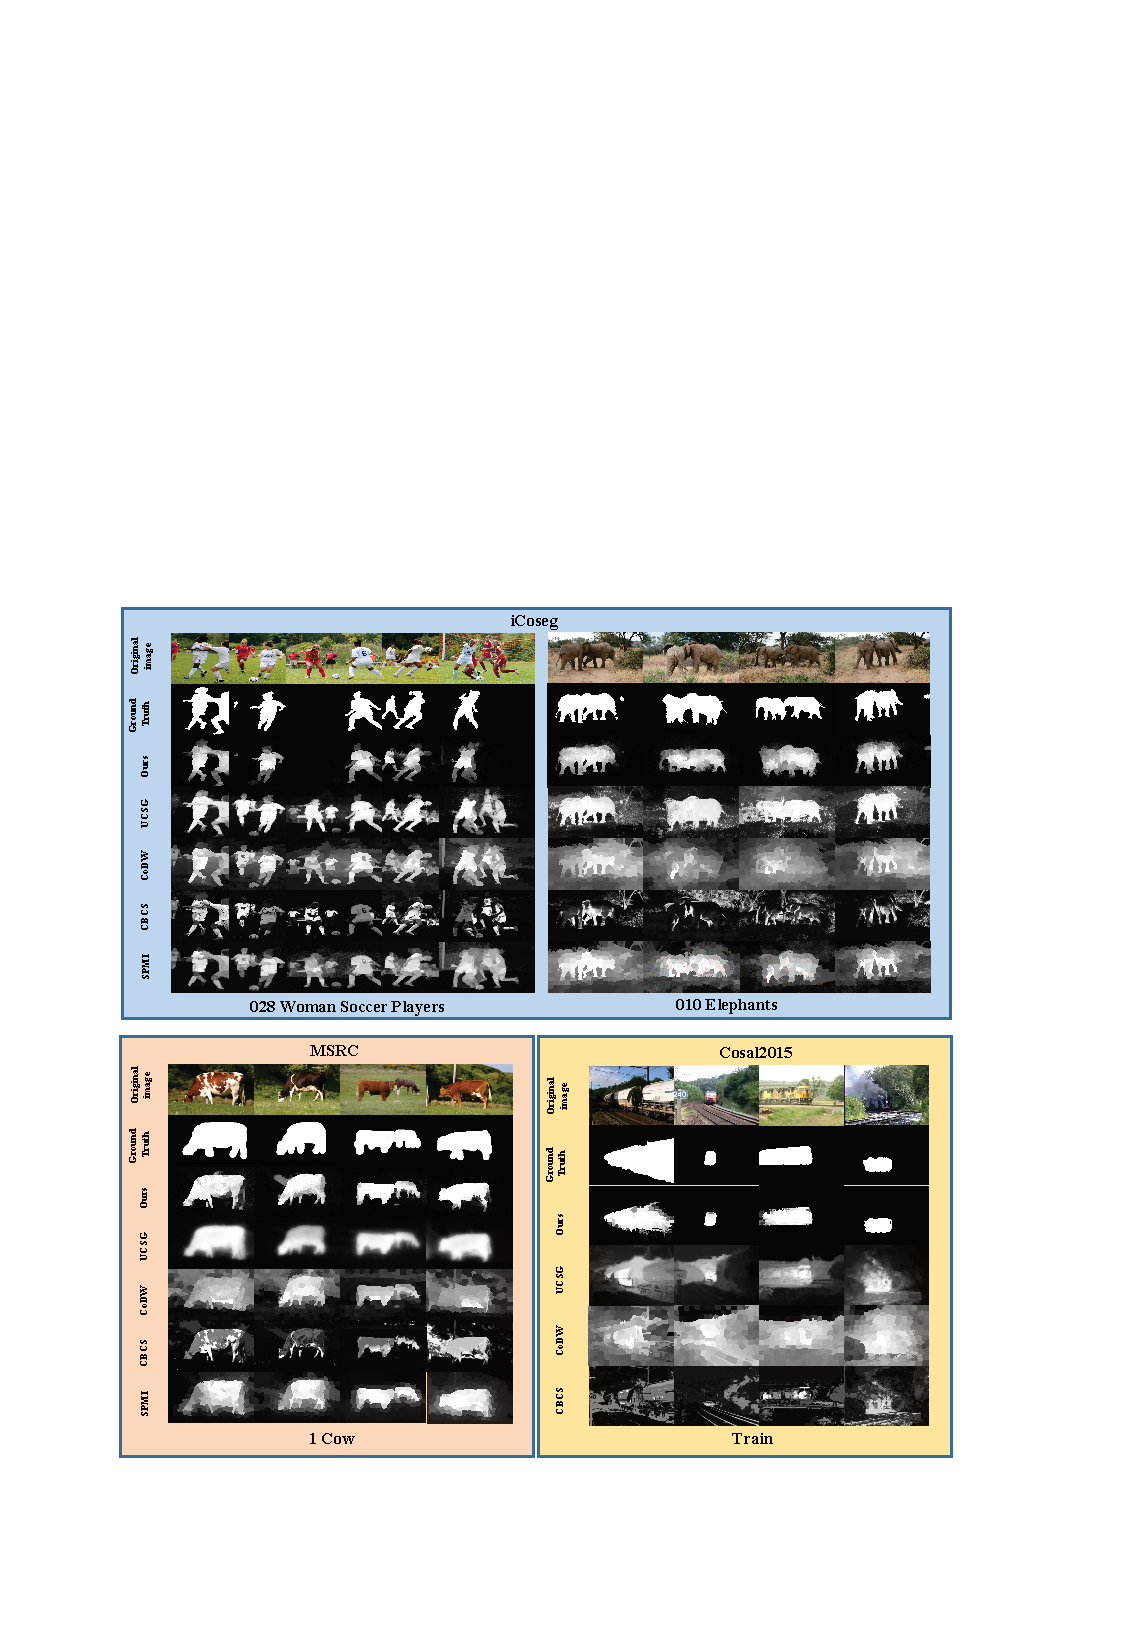
\includegraphics[scale=0.9]{Fig6.pdf}
\caption{Visual comparison between the proposed method and the other representative methods on three benchmark datasets.}
\vspace{-5pt}
\label{fig:label}
\end{figure*}

\subsection {Comparison with the State-of-the-Art}
With the evaluation criteria stated above, we compare the proposed method with other state-of-the-art co-saliency detection methods. SACS \cite{Cao2014}, CBCS \cite{Fu2013}, CSHS \cite{liu2014co},  CoDW \cite{Zhang2016}, CSSCF \cite{DBLP:journals/tmm/JerripothulaCY16}, and UCSG\cite{DBLP:conf/eccv/HsuTLQC18} are unsupervised methods. GW\cite{DBLP:conf/ijcai/WeiZBLW17}, SP-MIL \cite{zhang2017co} and FASS\cite{DBLP:conf/mm/ZhengZZ18} are data driven methods. For fair comparison, we only compare our method with methods which provide available saliency maps or executable implementations with their recommended parameter settings.

\noindent \textbf{Visual Comparison.} We show some experimental results in Fig.6 for subjective evaluation, which contains examples of four image groups, i.e., \textit{elephants} group and the\textit{ women soccer} group from iCoseg dataset, the\textit{ cattle} group from MSRC dataset, and the \textit{train} group from Cosal2015 dataset. As can be seen, compared with the state-of-the-art methods, our results can better suppress the common background. Our results can not only highlight the common objects with great appearance variations in semantic level (i.e., the cattle and trains), but also distinguish the co-salient objects(i.e., the white soccer players) from the non-common objects (i.e., the red soccer players) with low-level consistency. Moreover, our  method  produces better saliency maps both in terms of the accuracy of contours and discrimination of different objects, which helps to easily select a binarization threshold to segment out the foregrounds given a co-saliency map. The effectiveness of our method mainly results from hierarchical consistency: 1) By using the background consistency, our SVAE network can effectively distinguish the co-salient objects from the co-background. 2) By leveraging the capacity disparity of high-level and low-level features, our method can explore the multi-level salient objects consistency in complex scenarios to find the real co-saliency.


\begin{table*}[!tbp]
\caption{Quantitative comparison with the state-of-the-arts on three famous benchmark datasets.}
\begin{tabular}{c|c|ccc|ccc|ccc}
\toprule
\multirow{2}{*}{Method} & \multirow{2}{*}{Setting} & \multicolumn{3}{c|}{iCoseg}                      & \multicolumn{3}{c|}{MSRC}                        & \multicolumn{3}{c}{Cosal2015}                   \\ \cline{3-11} 
                        &                          & AP             & $F$              & $S$              & AP             & $F$              & $S$              & AP             & $F$              & $S$              \\ \hline
SACS                    & Unsupervised             & 0.840          & 0.733          & 0.753          & 0.860          & 0.757          & 0.716          & 0.708          & 0.632          & 0.697          \\
CBCS                    & Unsupervised             & 0.797          & 0.690          & 0.671          & 0.703          & 0.587          & 0.671          & 0.586          & 0.514          & 0.545          \\
CoDW                    & Unsupervised             & 0.877          & 0.699          & 0.751          & 0.843          & 0.593          & 0.718          & 0.744          & 0.560          & 0.650          \\
CSHS                    & Unsupervised             & 0.845          & 0.636          & 0.747          & 0.783          & 0.516          & 0.676          & 0.708          & 0.436          & 0.595          \\
CSSCF                   & Unsupervised             & 0.840          & 0.705          & 0.739          & 0.860          & 0.648          & 0.747          & 0.708          & 0.584          & 0.675          \\
UCSG                    & Unsupervised             & {\ul 0.911}    & {\ul 0.794}    & {\ul 0.822}    & {\ul 0.922}    & {\ul 0.792}    & {\ul 0.801}    & {\ul 0.815}    & {\ul 0.692}    & {\ul 0.754}    \\
Ours                    & Unsupervised             & \textbf{0.932} & \textbf{0.831} & \textbf{0.858} & \textbf{0.927} & \textbf{0.801} & \textbf{0.806} & \textbf{0.832} & \textbf{0.712} & \textbf{0.763} \\ \hline
SP-MIL                  & Data-Driven              & 0.874          & 0.703          & 0.782          & 0.853          & 0.625          & 0.775          & -              & -              & -              \\
GW                      & Data-Driven              & 0.890          & 0.751          & 0.780          & 0.896          & 0.705          & 0.737          & 0.800          & 0.661          & 0.745          \\
FASS                    & Data-Driven              & 0.930          & 0.838          & 0.867          & 0.925          & 0.808          & 0.804          & 0.810          & 0.696          & 0.802          \\ 
\bottomrule
\end{tabular}
\end{table*}\textbf{}


\noindent \textbf{Quantitative Comparison.} Fig. 5 shows the PR curves, table 1  contains the AP, F measure and S measure scores of ours and compared methods on three datasets. As can be seen in the PR curves, the proposed method consistently outperforms the state-of-the-arts, which shows that our co-saliency maps result in the highest precision/recall rates in the widest ranges of recall/false positive rates. In table 1, the proposed approach performs better than all unsupervised state-of-the-art methods in terms of all the performance metric on three datasets. For example, our method (the bold numbers) outperforms the second best results (the underlined numbers) \cite{DBLP:conf/eccv/HsuTLQC18} a large margin by $2.3\%$, $4.7\%$, and $4.4 \%$ in terms of AP, F measure and S measure respectively. Our method also outperforms the very recent state-of-the-art data driven methods SP-MIL and GW on three datasets.  And the proposed method achieves competitive performance compared to the data driven method FASS which products good results by leveraging the supervision information within the three test datasets. 

\noindent \textbf{Timing Comparison.} Table.2 lists the average execution time for each image by using different approaches.  Since the data driven methods need extra training time, we do not report their runtime performance. As can be seen, compared with other unsupervised methods, the proposed algorithm achieves a good performance with the moderate computational complexity. This indicates that the proposed method is efficient.



\begin{table}
  \caption{Average Runtime(s) Per Image}
  \label{tab:freq}
  \renewcommand\tabcolsep{4.5pt}
  \scalebox{0.85}{
\begin{tabular}{cccccccc}
    \toprule
Method       & SACS   & CBCS   & CoDW   & CSHS   & CSSCF  & UCSG   & Ours   \\     \midrule
RunTime & 7.4s   & 1.5s   & 6.5s   & 103.4s & 127.5s & 15.6s  & 6.8s   \\ \hline
Code         & Matlab & Matlab & Matlab & Matlab & Matlab & Matlab & Matlab \\   \bottomrule
\end{tabular}}
\end{table}



\subsection{Ablation Study}
In background consistency Mining, the Isolation Forest anomaly detection algorithm helps us decrease the incorrect  backgrounds rates from 10\%, 8\%, and 7\% to 3\%, 4.1\%, and 2.4\% in iCoseg, MSRC, and Cosal2015 datasets respectively. The true positive instances take 85\%, 75\%, and 80\% in the eliminated sets for three datasets. And we further examine the effectiveness of the proposed techniques by using five baselines on the challenging iCoseg dataset: Ours-NBC means without using the co-background in our framework; Ours-NSP means without using the structure perceptual (SP) loss in training SVAE; Ours-LOC means we only use the low-level features to mine salient objects consistency; Ours-HOC means we only use the high-level features to mine salient objects consistency; Ours-NF means without using the CRF based refinement in our framework. The quantitative results of these baselines can be seen in Figure7. It shows the increased performance benefits from the hierarchical consistency. The SVAE with the structure perceptual (SP) loss can better model the co-background and then distinguish the co-salient objects from the co-background. We also prove that neither low-level nor high-level consistency can individually handle all the cases in co-saliency detection. And with the refinement of CRF, the proposed method can generate more favorable and consistent co-saliency results.


\begin{figure}[!h]
\centering
\includegraphics[scale=0.6]{Fig71.pdf}
\caption{Evaluation of component effectiveness.}
\label{fig:label}
\end{figure}

\section{conclusions}
In this paper, we propose a novel co-saliency detection framework based on hierarchical consistency to alleviate the limitations in previous co-saliency detection methods. Our method integrates background consistency, high-level and low-level objects consistency in a unified framework. By designing a novel superpixel-wise variational autoencoder (SVAE) network, we precisely distinguish the salient objects from the background collection based on the reconstruction errors. Then, we propose a two-stage clustering strategy to explore the multi-level salient objects consistency by using high-level and low-level features separately. Finally, the co-saliency results are refined by applying a CRF based refinement method with the multi-level salient objects consistency. Extensive experiments on three widely datasets show that our method achieves superior or competitive performance compared to the state-of-the-art methods.












\bibliographystyle{ACM-Reference-Format}
\bibliography{sample-base}

% 
% If your work has an appendix, this is the place to put it.

\end{document}
